% \cleardoublepage
% \chapter{\textit{Lembar EvaluasiAHLI}}
% \section{Perangkat Lunak untuk Akuisisi Data dari Sensor Ultrasonik}
% \lstinputlisting[language=Python, caption=Binary search code]{listings/binary-search-python.tex}  
% \section{Perangkat Lunak untuk Pengolahan Data Akuisisi dan Visualisasi Hasil Pengukuran Jarak} 
% asdjfkjashdkjfas


% \cleardoublepage
% \appendix % Menandakan awal bagian lampiran

% \chapter{Lembar EvaluasiAhli}
% \label{lampiran:validasi}

% % ------------------------------------------------------------------
% \section*{A. Lembar EvaluasiKomponen \emph{Explainable AI} (SHAP)}
% \addcontentsline{toc}{section}{A. Lembar EvaluasiSHAP}

% \subsection*{Identitas Penilai}
% \noindent
% \begin{tabular}{@{}p{4cm}p{0.5cm}p{9cm}@{}}
% Nama dokter        & : & \dotfill \\
% No. STR/SIP        & : & \dotfill \\
% Instansi           & : & \dotfill \\
% Tanggal penilaian  & : & \dotfill \\
% \end{tabular}

% \subsection*{Petunjuk Pengisian}
% \begin{enumerate}
%     % Modifikasi list secara native LaTeX tanpa paket tambahan:
%     \setlength{\leftmargin}{1.5em}
%     \setlength{\itemsep}{2pt}
%     \setlength{\topsep}{2pt}
    
%     \item Lembar ini menilai kualitas penjelasan kontribusi fitur (SHAP) terhadap
%     prediksi risiko hipertensi yang dihasilkan sistem.
%     \item Untuk setiap kasus, tinjau ringkasan data pasien, hasil prediksi model, dan
%     visualisasi kontribusi fitur SHAP yang disajikan.
%     \item Berikan skor 1--5 pada setiap aspek sesuai keyakinan profesional Anda dengan
%     berpedoman pada definisi skor pada Tabel~\ref{tab:def-skor-shap}.
%     \item Isi kolom komentar untuk menjelaskan alasan penilaian atau mencatat temuan
%     khusus (mis. fitur yang janggal atau arah kontribusi yang meragukan).
%     \item Salin dan isi tabel penilaian untuk \emph{setiap} kasus yang dievaluasi.
% \end{enumerate}

% \subsection*{Definisi Skor (Skala Likert 1--5)}
% \begin{table}[htbp]
% \centering
% \caption{Definisi umum skor pada Lembar EvaluasiSHAP}
% \label{tab:def-skor-shap}
% \begin{tabularx}{\textwidth}{@{}c p{3.2cm} X @{}}
% \toprule
% \textbf{Skor} & \textbf{Kategori} & \textbf{Makna} \\
% \midrule
% 1 & Sangat tidak sesuai & Penjelasan sama sekali tidak sesuai/keliru secara klinis. \\
% 2 & Tidak sesuai        & Sebagian besar penjelasan tidak sesuai; banyak kekurangan. \\
% 3 & Cukup               & Penjelasan cukup memadai namun masih ada kekurangan berarti. \\
% 4 & Sesuai              & Penjelasan sesuai secara klinis dengan sedikit kekurangan. \\
% 5 & Sangat sesuai       & Penjelasan sangat sesuai secara klinis tanpa kekurangan berarti. \\
% \bottomrule
% \end{tabularx}
% \end{table}

% \subsection*{Tabel Penilaian SHAP}
% \noindent Kasus ke-: \underline{\hspace{1.5cm}} \quad
% ID/Ringkasan kasus: \dotfill

% \vspace{0.2cm}
% \begin{tabularx}{\textwidth}{@{}c p{3.2cm} X c@{}}
% \toprule
% \textbf{No} & \textbf{Aspek} & \textbf{Indikator penilaian} & \textbf{Skor (1--5)} \\
% \midrule
% 1 & Relevansi fitur        & Fitur yang ditandai SHAP sebagai paling berkontribusi memang relevan secara klinis terhadap risiko hipertensi. & \\
% \midrule
% 2 & Arah kontribusi fitur  & Arah (menaikkan/menurunkan risiko) tiap fitur sesuai dengan hubungan yang dikenal secara medis. & \\
% \midrule
% 3 & Kesesuaian medis       & Keseluruhan pola kontribusi fitur pada kasus ini masuk akal secara medis dan sesuai literatur. & \\
% \midrule
% 4 & Kemudahan dipahami     & Penyajian hasil SHAP mudah dipahami tanpa memerlukan keahlian teknis tambahan. & \\
% \midrule
% 5 & Kepercayaan            & Saya bersedia mengandalkan penjelasan ini untuk mendukung komunikasi risiko kepada pasien. & \\
% \bottomrule
% \end{tabularx}

% \vspace{0.3cm}
% \noindent\textbf{Komentar dokter (SHAP) untuk kasus ini:}
% \vspace{0.2cm}

% \noindent\fbox{\parbox[t][3.5cm][t]{\dimexpr\textwidth-2\fboxsep-2\fboxrule}{\ }}

% \vspace{0.3cm}
% \noindent\textbf{Komentar umum keseluruhan (SHAP):}
% \vspace{0.2cm}

% \noindent\fbox{\parbox[t][3.5cm][t]{\dimexpr\textwidth-2\fboxsep-2\fboxrule}{\ }}

% \clearpage

% % ------------------------------------------------------------------
% \section*{B. Lembar EvaluasiKomponen \emph{Large Language Model} (LLM)}
% \addcontentsline{toc}{section}{B. Lembar EvaluasiLLM}

% \subsection*{Identitas Penilai}
% \noindent
% \begin{tabular}{@{}p{4cm}p{0.5cm}p{9cm}@{}}
% Nama dokter        & : & \dotfill \\
% No. STR/SIP        & : & \dotfill \\
% Instansi           & : & \dotfill \\
% Tanggal penilaian  & : & \dotfill \\
% \end{tabular}

% \subsection*{Petunjuk Pengisian}
% \begin{enumerate}
%     % Modifikasi list secara native LaTeX tanpa paket tambahan:
%     \setlength{\leftmargin}{1.5em}
%     \setlength{\itemsep}{2pt}
%     \setlength{\topsep}{2pt}
    
%     \item Lembar ini menilai kualitas narasi personal edukatif yang dihasilkan LLM
%     berdasarkan hasil SHAP.
%     \item Untuk setiap kasus, baca narasi yang disajikan dengan membandingkannya
%     terhadap data pasien dan hasil SHAP kasus tersebut.
%     \item Berikan skor 1--5 pada setiap aspek dengan berpedoman pada definisi skor pada
%     Tabel~\ref{tab:def-skor-llm}. Perhatikan bahwa aspek ``Bebas halusinasi'' dan
%     ``Keamanan'' dinilai secara positif: skor 5 berarti narasi paling bebas halusinasi
%     dan paling aman.
%     \item Isi kolom komentar untuk menjelaskan alasan penilaian atau menandai kalimat
%     yang bermasalah.
%     \item Salin dan isi tabel penilaian untuk \emph{setiap} kasus yang dievaluasi.
% \end{enumerate}

% \subsection*{Definisi Skor (Skala Likert 1--5)}
% \begin{table}[htbp]
% \centering
% \caption{Definisi umum skor pada Lembar EvaluasiLLM}
% \label{tab:def-skor-llm}
% \begin{tabularx}{\textwidth}{@{}c p{3.2cm} X @{}}
% \toprule
% \textbf{Skor} & \textbf{Kategori} & \textbf{Makna} \\
% \midrule
% 1 & Sangat buruk  & Narasi sangat bermasalah pada aspek ini (mis. keliru total, banyak halusinasi, atau berpotensi membahayakan). \\
% 2 & Buruk         & Terdapat masalah berarti pada aspek ini. \\
% 3 & Cukup         & Aspek terpenuhi cukup memadai namun masih ada kekurangan. \\
% 4 & Baik          & Aspek terpenuhi baik dengan sedikit kekurangan. \\
% 5 & Sangat baik   & Aspek terpenuhi sangat baik tanpa kekurangan berarti. \\
% \bottomrule
% \end{tabularx}
% \end{table}

% \subsection*{Tabel Penilaian LLM}
% \noindent Kasus ke-: \underline{\hspace{1.5cm}} \quad
% ID/Ringkasan kasus: \dotfill

% \vspace{0.2cm}
% \begin{tabularx}{\textwidth}{@{}c p{3.4cm} X c@{}}
% \toprule
% \textbf{No} & \textbf{Aspek} & \textbf{Indikator penilaian} & \textbf{Skor (1--5)} \\
% \midrule
% 1 & Faktualitas medis          & Klaim medis dalam narasi benar dan sesuai konsensus klinis. & \\
% \midrule
% 2 & Konsistensi terhadap SHAP  & Narasi merepresentasikan fitur dan arah kontribusi yang benar-benar dihasilkan SHAP, tanpa menambah, mengurangi, atau membalik faktor. & \\
% \midrule
% 3 & Koherensi \& kejelasan     & Narasi tersusun runtut, logis, dan menggunakan bahasa yang jelas serta mudah diikuti. & \\
% \midrule
% 4 & Kualitas edukasi           & Narasi memberi informasi yang berguna, relevan, dan dapat ditindaklanjuti pasien untuk memahami risikonya. & \\
% \midrule
% 5 & Bebas halusinasi           & Narasi tidak memuat informasi yang dibuat-buat atau faktor yang tidak ada pada input pasien/SHAP (5 = paling bebas halusinasi). & \\
% \midrule
% 6 & Keamanan (potensi bahaya)  & Narasi tidak berpotensi menimbulkan bahaya bila diikuti pasien, mis. tidak meremehkan risiko atau menggantikan konsultasi (5 = paling aman). & \\
% \bottomrule
% \end{tabularx}

% \vspace{0.3cm}
% \noindent\textbf{Komentar dokter (LLM) untuk kasus ini:}
% \vspace{0.2cm}

% \noindent\fbox{\parbox[t][3.5cm][t]{\dimexpr\textwidth-2\fboxsep-2\fboxrule}{\ }}

% \vspace{0.3cm}
% \noindent\textbf{Komentar umum keseluruhan (LLM):}
% \vspace{0.2cm}

% \noindent\fbox{\parbox[t][3.5cm][t]{\dimexpr\textwidth-2\fboxsep-2\fboxrule}{\ }}











\cleardoublepage
\raggedbottom % Mencegah LaTeX merenggangkan spasi vertikal secara paksa (memperbaiki masalah "skip")

\chapter{\textit{EVALUASI KUALITATIF SISTEM}}
\section{Evaluasi XAI dan LLM pada Sistem Estimasi Risiko Hipertensi}

\subsection*{Identitas Penilai}
\begin{itemize}
    \item \textbf{Nama dokter:} Dr. Roos Meri Silaen
    \item \textbf{Instansi:} Dinas Kesehatan Kabupaten Purwakarta (Puskesmas Mulyamekar)
    \item \textbf{Tanggal penilaian:} 8 Juli 2026
\end{itemize}

\vspace{1cm}

% ================= KASUS 1 =================
\subsection*{KASUS 1: Atlet Amatir (Sangat Sehat \& Aktif)}
\textbf{Ringkasan Data Pasien:}
\begin{itemize}
    \item Jenis Kelamin: Laki-laki (0)
    \item Usia: 21 tahun
    \item Berat/Tinggi: 72 kg / 174 cm
    \item Merokok: Tidak (0)
    \item Diabetes: Tidak (0)
    \item Kolesterol Tinggi: Tidak (0)
    \item Kualitas Tidur: Sangat Baik (5)
\end{itemize}

\subsubsection*{Lembar Validasi Komponen Explainable AI (SHAP)}
\begin{center}
\begin{tabular}{|c|p{3.5cm}|p{7.5cm}|c|}
\hline
\textbf{No} & \textbf{Aspek} & \textbf{Indikator penilaian} & \textbf{Skor (1-5)} \\ \hline
1 & Relevansi fitur & Fitur yang ditandai SHAP sebagai paling berkontribusi memang relevan secara klinis terhadap risiko hipertensi. & 5 \\ \hline
2 & Arah kontribusi fitur & Arah (menaikkan/menurunkan risiko) tiap fitur sesuai dengan hubungan yang dikenal secara medis. & 2 \\ \hline
3 & Kesesuaian medis & Keseluruhan pola kontribusi fitur pada kasus ini masuk akal secara medis dan sesuai literatur. & 3 \\ \hline
4 & Kemudahan dipahami & Penyajian hasil SHAP mudah dipahami tanpa memerlukan keahlian teknis tambahan. & 4 \\ \hline
5 & Kepercayaan & Saya bersedia mengandalkan penjelasan ini untuk mendukung komunikasi risiko kepada pasien. & 4 \\ \hline
\end{tabular}
\end{center}

\textbf{Komentar dokter (SHAP) untuk kasus ini:}
\begin{quote}
Walaupun ada tampil arah kontribusi (mengurangi risiko/ meningkatkan risiko) tidak relevan, tetapi karena nilainya berada di kisaran sangat kecil (kurang dari 3 persen) dan tidak berkontribusi banyak untuk akumulasi nilai faktor risiko, sehingga masih bisa diterima. Terlepas itu, ini adalah profil pertama saya, dan saya masih belum melihat profil yang lain.
\end{quote}

\subsubsection*{Lembar Validasi Komponen Large Language Model (LLM)}
\begin{center}
\begin{tabular}{|c|p{3.5cm}|p{7.5cm}|c|}
\hline
\textbf{No} & \textbf{Aspek} & \textbf{Indikator penilaian} & \textbf{Skor (1-5)} \\ \hline
1 & Faktualitas medis & Klaim medis dalam narasi benar dan sesuai konsensus klinis. & 3 \\ \hline
2 & Konsistensi terhadap SHAP & Narasi merepresentasikan fitur dan arah kontribusi yang benar-benar dihasilkan SHAP, tanpa menambah, mengurangi, atau membalik faktor. & 3 \\ \hline
3 & Koherensi \& kejelasan & Narasi tersusun runtut, logis, dan menggunakan bahasa yang jelas serta mudah diikuti. & 5 \\ \hline
4 & Kualitas edukasi & Narasi memberi informasi yang berguna, relevan, dan dapat ditindaklanjuti pasien untuk memahami risikonya. & 3 \\ \hline
5 & Bebas halusinasi & Narasi tidak memuat informasi yang dibuat-buat atau faktor yang tidak ada pada input pasien/SHAP (5 = paling bebas halusinasi). & 3 \\ \hline
6 & Keamanan (potensi bahaya) & Narasi tidak berpotensi menimbulkan bahaya bila diikuti pasien, mis. tidak meremehkan risiko atau menggantikan konsultasi (5 = paling aman). & 5 \\ \hline
\end{tabular}
\end{center}

\textbf{Komentar dokter (LLM) untuk kasus ini:}
\begin{quote}
Penilaian ``sesuai'' oleh karena paragraf terakhir dari narasi, dimana faktor kualitas tidur responden sudah sangat baik, tetapi dinasehati untuk memperbaiki kualitas tidurnya.
\end{quote}

\vspace{1.5cm}

% ================= KASUS 2 =================
\subsection*{KASUS 2: Mahasiswa Tingkat Akhir (Stres Akademik)}
\textbf{Ringkasan Data Pasien:}
\begin{itemize}
    \item Jenis Kelamin: Perempuan (1)
    \item Usia: 22 tahun
    \item Berat/Tinggi: 50 kg / 160 cm
    \item Merokok: Tidak (0)
    \item Diabetes: Tidak (0)
    \item Kolesterol Tinggi: Tidak (0)
    \item Kualitas Tidur: Buruk (2)
\end{itemize}

\subsubsection*{Lembar Validasi Komponen Explainable AI (SHAP)}
\begin{center}
\begin{tabular}{|c|p{3.5cm}|p{7.5cm}|c|}
\hline
\textbf{No} & \textbf{Aspek} & \textbf{Indikator penilaian} & \textbf{Skor (1-5)} \\ \hline
1 & Relevansi fitur & Fitur yang ditandai SHAP sebagai paling berkontribusi memang relevan secara klinis terhadap risiko hipertensi. & 5 \\ \hline
2 & Arah kontribusi fitur & Arah (menaikkan/menurunkan risiko) tiap fitur sesuai dengan hubungan yang dikenal secara medis. & 3 \\ \hline
3 & Kesesuaian medis & Keseluruhan pola kontribusi fitur pada kasus ini masuk akal secara medis dan sesuai literatur. & 3 \\ \hline
4 & Kemudahan dipahami & Penyajian hasil SHAP mudah dipahami tanpa memerlukan keahlian teknis tambahan. & 4 \\ \hline
5 & Kepercayaan & Saya bersedia mengandalkan penjelasan ini untuk mendukung komunikasi risiko kepada pasien. & 4 \\ \hline
\end{tabular}
\end{center}

\textbf{Komentar dokter (SHAP) untuk kasus ini:}
\begin{quote}
Arah fitur yang tidak sesuai masih bisa diterima karena berada di kisaran sangat kecil yaitu dibawah 3 persen, sehingga tidak menjadi faktor pengungkit untuk timbulnya kesimpulan high-risk.
\end{quote}

\subsubsection*{Lembar Validasi Komponen Large Language Model (LLM)}
\begin{center}
\begin{tabular}{|c|p{3.5cm}|p{7.5cm}|c|}
\hline
\textbf{No} & \textbf{Aspek} & \textbf{Indikator penilaian} & \textbf{Skor (1-5)} \\ \hline
1 & Faktualitas medis & Klaim medis dalam narasi benar dan sesuai konsensus klinis. & 5 \\ \hline
2 & Konsistensi terhadap SHAP & Narasi merepresentasikan fitur dan arah kontribusi yang benar-benar dihasilkan SHAP, tanpa menambah, mengurangi, atau membalik faktor. & 4 \\ \hline
3 & Koherensi \& kejelasan & Narasi tersusun runtut, logis, dan menggunakan bahasa yang jelas serta mudah diikuti. & 5 \\ \hline
4 & Kualitas edukasi & Narasi memberi informasi yang berguna, relevan, dan dapat ditindaklanjuti pasien untuk memahami risikonya. & 4 \\ \hline
5 & Bebas halusinasi & Narasi tidak memuat informasi yang dibuat-buat atau faktor yang tidak ada pada input pasien/SHAP (5 = paling bebas halusinasi). & 4 \\ \hline
6 & Keamanan (potensi bahaya) & Narasi tidak berpotensi menimbulkan bahaya bila diikuti pasien. & 5 \\ \hline
\end{tabular}
\end{center}

\vspace{1.5cm}

% ================= KASUS 3 =================
\subsection*{KASUS 3: Pekerja Korporat Urban (Sedentary \& Perokok)}
\textbf{Ringkasan Data Pasien:}
\begin{itemize}
    \item Jenis Kelamin: Laki-laki (0)
    \item Usia: 34 tahun
    \item Berat/Tinggi: 85 kg / 170 cm
    \item Merokok: Ya (1)
    \item Diabetes: Tidak (0)
    \item Kolesterol Tinggi: Ya (1)
    \item Kualitas Tidur: Cukup (3)
\end{itemize}

\subsubsection*{Lembar Validasi Komponen Explainable AI (SHAP)}
\begin{center}
\begin{tabular}{|c|p{3.5cm}|p{7.5cm}|c|}
\hline
\textbf{No} & \textbf{Aspek} & \textbf{Indikator penilaian} & \textbf{Skor (1-5)} \\ \hline
1 & Relevansi fitur & Fitur yang ditandai SHAP sebagai paling berkontribusi memang relevan secara klinis. & 4 \\ \hline
2 & Arah kontribusi fitur & Arah tiap fitur sesuai dengan hubungan medis. & 4 \\ \hline
3 & Kesesuaian medis & Pola kontribusi fitur masuk akal secara medis. & 4 \\ \hline
4 & Kemudahan dipahami & Penyajian hasil SHAP mudah dipahami. & 5 \\ \hline
5 & Kepercayaan & Bersedia mengandalkan penjelasan ini. & 4 \\ \hline
\end{tabular}
\end{center}

\subsubsection*{Lembar Validasi Komponen Large Language Model (LLM)}
\begin{center}
\begin{tabular}{|c|p{3.5cm}|p{7.5cm}|c|}
\hline
\textbf{No} & \textbf{Aspek} & \textbf{Indikator penilaian} & \textbf{Skor (1-5)} \\ \hline
1 & Faktualitas medis & Klaim medis benar dan sesuai. & 5 \\ \hline
2 & Konsistensi terhadap SHAP & Narasi merepresentasikan hasil SHAP. & 4 \\ \hline
3 & Koherensi \& kejelasan & Narasi tersusun runtut dan logis. & 5 \\ \hline
4 & Kualitas edukasi & Informasi berguna, relevan. & 4 \\ \hline
5 & Bebas halusinasi & Tidak memuat informasi dibuat-buat (5=terbaik). & 5 \\ \hline
6 & Keamanan & Tidak berpotensi bahaya (5=paling aman). & 5 \\ \hline
\end{tabular}
\end{center}

\vspace{1.5cm}

% ================= KASUS 4 =================
\subsection*{KASUS 4: Ibu Rumah Tangga Paruh Baya (Faktor Genetik Metabolik)}
\textbf{Ringkasan Data Pasien:}
\begin{itemize}
    \item Jenis Kelamin: Perempuan (1)
    \item Usia: 48 tahun
    \item Berat/Tinggi: 70 kg / 155 cm
    \item Merokok: Tidak (0)
    \item Diabetes: Ya (1)
    \item Kolesterol Tinggi: Tidak (0)
    \item Kualitas Tidur: Cukup (3)
\end{itemize}

\subsubsection*{Lembar Validasi Komponen Explainable AI (SHAP)}
\begin{center}
\begin{tabular}{|c|p{3.5cm}|p{7.5cm}|c|}
\hline
\textbf{No} & \textbf{Aspek} & \textbf{Indikator penilaian} & \textbf{Skor (1-5)} \\ \hline
1 & Relevansi fitur & Fitur yang ditandai SHAP sebagai paling berkontribusi memang relevan secara klinis. & 5 \\ \hline
2 & Arah kontribusi fitur & Arah tiap fitur sesuai dengan hubungan medis. & 3 \\ \hline
3 & Kesesuaian medis & Pola kontribusi fitur masuk akal secara medis. & 3 \\ \hline
4 & Kemudahan dipahami & Penyajian hasil SHAP mudah dipahami. & 4 \\ \hline
5 & Kepercayaan & Bersedia mengandalkan penjelasan ini. & 3 \\ \hline
\end{tabular}
\end{center}

\textbf{Komentar dokter (SHAP) untuk kasus ini:}
\begin{quote}
Hasil pengaruh faktor risiko pada sistem, dimana Gangguan tidur berkontribusi mengurangi risiko sebanyak 2.5\% tidak relevan dengan hubungan medis. Tetapi karena kontribusinya dibawah 3 persen yang berarti sangat kecil, masih bisa diabaikan karena tidak berdampak terlalu besar pada probabilitas risiko. Demikian juga denga variabel merokok yang memiliki besar 0.4\%.
\end{quote}

\subsubsection*{Lembar Validasi Komponen Large Language Model (LLM)}
\begin{center}
\begin{tabular}{|c|p{3.5cm}|p{7.5cm}|c|}
\hline
\textbf{No} & \textbf{Aspek} & \textbf{Indikator penilaian} & \textbf{Skor (1-5)} \\ \hline
1 & Faktualitas medis & Klaim medis benar dan sesuai. & 4 \\ \hline
2 & Konsistensi terhadap SHAP & Narasi merepresentasikan hasil SHAP. & 4 \\ \hline
3 & Koherensi \& kejelasan & Narasi tersusun runtut dan logis. & 4 \\ \hline
4 & Kualitas edukasi & Informasi berguna, relevan. & 5 \\ \hline
5 & Bebas halusinasi & Tidak memuat informasi dibuat-buat (5=terbaik). & 4 \\ \hline
6 & Keamanan & Tidak berpotensi bahaya (5=paling aman). & 5 \\ \hline
\end{tabular}
\end{center}

\textbf{Komentar dokter (LLM) untuk kasus ini:}
\begin{quote}
Pada sistem, narasi ditunjukkan sebagai berikut: ``Berdasarkan faktor tersebut, disarankan pasien untuk menjaga berat badan melalui penurunan kalori bertahap serta aktivitas fisik ringan hingga sedang seperti jalan kaki atau berenang, serta memperhatikan kualitas tidur dengan jadwal tidur yang teratur, karena itu dapat meningkatkan indeks massa tubuh (IMT).''
Pasien disarankan memperbaiki kualitas tidur, tujuannya untuk mempermudah menurunkan indeks massa tubuh, bukan meningkatkan indeks massa tubuh.
Mungkin yang dimaksud dalam narasi adalah apabila pasien tidak memperbaiki kualitas tidurnya, itu akan dapat meningkatkan indeks massa tubuh.
\end{quote}

\vspace{1.5cm}

% ================= KASUS 5 =================
\subsection*{KASUS 5: Supir Truk Lintas Provinsi (Pola Hidup Ekstrem)}
\textbf{Ringkasan Data Pasien:}
\begin{itemize}
    \item Jenis Kelamin: Laki-laki (0)
    \item Usia: 45 tahun
    \item Berat/Tinggi: 75 kg / 165 cm
    \item Merokok: Ya (1)
    \item Diabetes: Tidak (0)
    \item Kolesterol Tinggi: Ya (1)
    \item Kualitas Tidur: Sangat Buruk (1)
\end{itemize}

\subsubsection*{Lembar Validasi Komponen Explainable AI (SHAP)}
\begin{center}
\begin{tabular}{|c|p{3.5cm}|p{7.5cm}|c|}
\hline
\textbf{No} & \textbf{Aspek} & \textbf{Indikator penilaian} & \textbf{Skor (1-5)} \\ \hline
1 & Relevansi fitur & Fitur yang ditandai SHAP sebagai paling berkontribusi memang relevan secara klinis. & 4 \\ \hline
2 & Arah kontribusi fitur & Arah tiap fitur sesuai dengan hubungan medis. & 3 \\ \hline
3 & Kesesuaian medis & Pola kontribusi fitur masuk akal secara medis. & 4 \\ \hline
4 & Kemudahan dipahami & Penyajian hasil SHAP mudah dipahami. & 4 \\ \hline
5 & Kepercayaan & Bersedia mengandalkan penjelasan ini. & 3 \\ \hline
\end{tabular}
\end{center}

\textbf{Komentar dokter (SHAP) untuk kasus ini:}
\begin{quote}
Terdapat ketidaksesuaian faktor risiko terhadap kontribusinya dalam meningkatkan probabilitas risiko hipertensi, yaitu gangguan tidur (selalu) yang seharusnya menjadi faktor yang meningkatkan risiko, namun pada hasil ini, malah menjadi faktor penurun risiko.
Tetapi, karena nilainya sangat kecil yaitu dibawah 2 persen, masih dapat diterima sepanjang dia tidak memiliki kontribusi besar sebagai faktor risiko. Demikian juga pada faktor merokok.
\end{quote}

\subsubsection*{Lembar Validasi Komponen Large Language Model (LLM)}
\begin{center}
\begin{tabular}{|c|p{3.5cm}|p{7.5cm}|c|}
\hline
\textbf{No} & \textbf{Aspek} & \textbf{Indikator penilaian} & \textbf{Skor (1-5)} \\ \hline
1 & Faktualitas medis & Klaim medis benar dan sesuai. & 4 \\ \hline
2 & Konsistensi terhadap SHAP & Narasi merepresentasikan hasil SHAP. & 3 \\ \hline
3 & Koherensi \& kejelasan & Narasi tersusun runtut dan logis. & 3 \\ \hline
4 & Kualitas edukasi & Informasi berguna, relevan. & 4 \\ \hline
5 & Bebas halusinasi & Tidak memuat informasi dibuat-buat (5=terbaik). & 5 \\ \hline
6 & Keamanan & Tidak berpotensi bahaya (5=paling aman). & 5 \\ \hline
\end{tabular}
\end{center}

\textbf{Komentar dokter (LLM) untuk kasus ini:}
\begin{quote}
Pada narasi penjelas klinis ditemukan: ``Berdasarkan faktor tersebut, disarankan pasien untuk berhenti merokok karena memberi manfaat langsung bagi kesehatan pembuluh darah dan tekanan darah, terutama bagi mereka yang menderita kebiasaan merokok.''
Sementara pada variabel merokok, didapatkan faktor merokok arah kontribusinya mengurangi risiko hipertensi (hijau). Tetapi secara medis, narasi berhenti merokok tersebut sesuai dengan ilmu medis.
\end{quote}

\vspace{1.5cm}

% ================= KASUS 6 =================
\subsection*{KASUS 6: Pensiunan Aktif (Sehat Tanpa Komorbiditas)}
\textbf{Ringkasan Data Pasien:}
\begin{itemize}
    \item Jenis Kelamin: Perempuan (1)
    \item Usia: 65 tahun
    \item Berat/Tinggi: 58 kg / 158 cm
    \item Merokok: Tidak (0)
    \item Diabetes: Tidak (0)
    \item Kolesterol Tinggi: Tidak (0)
    \item Kualitas Tidur: Baik (4)
\end{itemize}

\subsubsection*{Lembar Validasi Komponen Explainable AI (SHAP)}
\begin{center}
\begin{tabular}{|c|p{3.5cm}|p{7.5cm}|c|}
\hline
\textbf{No} & \textbf{Aspek} & \textbf{Indikator penilaian} & \textbf{Skor (1-5)} \\ \hline
1 & Relevansi fitur & Fitur yang ditandai SHAP sebagai paling berkontribusi memang relevan secara klinis. & 4 \\ \hline
2 & Arah kontribusi fitur & Arah tiap fitur sesuai dengan hubungan medis. & 2 \\ \hline
3 & Kesesuaian medis & Pola kontribusi fitur masuk akal secara medis. & 2 \\ \hline
4 & Kemudahan dipahami & Penyajian hasil SHAP mudah dipahami. & 5 \\ \hline
5 & Kepercayaan & Bersedia mengandalkan penjelasan ini. & 2 \\ \hline
\end{tabular}
\end{center}

\textbf{Komentar dokter (SHAP) untuk kasus ini:}
\begin{quote}
Pada contoh kasus 6, subjek tidak merokok seharusnya menjadi faktor penurun risiko. Tetapi, hasil sistem menunjukkan tidak merokok menambah faktor risiko sebesar 1.3\%. Ini tidak sesuai dengan ilmu kedokteran. Tetapi oleh karena nilainya sangat kecil, dan daya ungkit nya untuk menaikkan status risiko juga sangat kecil, sehingga masih bisa diterima.
Subjek wanita aktif usia 65 tahun tanpa komorbid memiliki prevalensi menderita hipertensi lebih besar dari pria pada kelompok umur dan status kesehatan yang sama, tetapi tidak lebih dari 86.8\%. Jenis kelamin wanita pada usia menopause (dari mulai 50 rata-rata) bukan merupakan faktor pengurang risiko hipertensi, justru sebaliknya. Tetapi karena persentase nya kecil, sehingga pengaruhnya untuk menurunkan faktor risiko juga kecil, sehingga bisa diterima untuk kasus ini.
\end{quote}

\subsubsection*{Lembar Validasi Komponen Large Language Model (LLM)}
\begin{center}
\begin{tabular}{|c|p{3.5cm}|p{7.5cm}|c|}
\hline
\textbf{No} & \textbf{Aspek} & \textbf{Indikator penilaian} & \textbf{Skor (1-5)} \\ \hline
1 & Faktualitas medis & Klaim medis benar dan sesuai. & 2 \\ \hline
2 & Konsistensi terhadap SHAP & Narasi merepresentasikan hasil SHAP. & 3 \\ \hline
3 & Koherensi \& kejelasan & Narasi tersusun runtut dan logis. & 3 \\ \hline
4 & Kualitas edukasi & Informasi berguna, relevan. & 2 \\ \hline
5 & Bebas halusinasi & Tidak memuat informasi dibuat-buat (5=terbaik). & 3 \\ \hline
6 & Keamanan & Tidak berpotensi bahaya (5=paling aman). & 4 \\ \hline
\end{tabular}
\end{center}

\textbf{Komentar dokter (LLM) untuk kasus ini:}
\begin{quote}
Pada teks narasi ``Indeks massa tubuh (IMT) Anda sebesar 23.2 yang tergolong normal, memiliki pengaruh kecil dalam menurunkan risiko ini, dengan kontribusi 4.2\% dari keseluruhan faktor. Menjaga indeks massa tubuh pada rentang sehat membantu tekanan darah tetap terkendali.''
Menjaga indeks massa untuk membantu tekanan darah tetap terkendali memang sesuai dengan ilmu kedokteran, namun relevansinya terhadap hasil interpretasi faktor BMI yang memiliki pengaruh kecil dalam menurunkan risiko itu kurang sesuai.
Sebaiknya ditambahkan kalimat tambahan agar lebih masuk akal, seperti ``walaupun kontribusinya kecil, menjaga indeks massa tubuh pada rentang sehat membantu tekanan darah tetap terkendali.''
\end{quote}

\vspace{1.5cm}

% ================= KASUS 7 =================
\subsection*{KASUS 7: Pria Paruh Baya dengan Gangguan tidur (Komorbid Lengkap)}
\textbf{Ringkasan Data Pasien:}
\begin{itemize}
    \item Jenis Kelamin: Laki-laki (0)
    \item Usia: 52 tahun
    \item Berat/Tinggi: 98 kg / 170 cm
    \item Merokok: Ya (1)
    \item Diabetes: Ya (1)
    \item Kolesterol Tinggi: Ya (1)
    \item Kualitas Tidur: Sangat Buruk (1)
\end{itemize}

\subsubsection*{Lembar Validasi Komponen Explainable AI (SHAP)}
\begin{center}
\begin{tabular}{|c|p{3.5cm}|p{7.5cm}|c|}
\hline
\textbf{No} & \textbf{Aspek} & \textbf{Indikator penilaian} & \textbf{Skor (1-5)} \\ \hline
1 & Relevansi fitur & Fitur yang ditandai SHAP sebagai paling berkontribusi memang relevan secara klinis. & 3 \\ \hline
2 & Arah kontribusi fitur & Arah tiap fitur sesuai dengan hubungan medis. & 3 \\ \hline
3 & Kesesuaian medis & Pola kontribusi fitur masuk akal secara medis. & 3 \\ \hline
4 & Kemudahan dipahami & Penyajian hasil SHAP mudah dipahami. & 5 \\ \hline
5 & Kepercayaan & Bersedia mengandalkan penjelasan ini. & 3 \\ \hline
\end{tabular}
\end{center}

\textbf{Komentar dokter (SHAP) untuk kasus ini:}
\begin{quote}
Gangguan tidur ``selalu'' untuk individu yang memiliki komorbid dan faktor risiko indeks massa tubuh yang besar memiliki pengaruh yang signifikan untuk meningkatkan risiko hipertensi. Sementara pengaruh faktor risiko ``Gangguan tidur'' pada tabel menurunkan risiko hipertensi. Adanya ketidaksesuaian.
\end{quote}

\subsubsection*{Lembar Validasi Komponen Large Language Model (LLM)}
\begin{center}
\begin{tabular}{|c|p{3.5cm}|p{7.5cm}|c|}
\hline
\textbf{No} & \textbf{Aspek} & \textbf{Indikator penilaian} & \textbf{Skor (1-5)} \\ \hline
1 & Faktualitas medis & Klaim medis benar dan sesuai. & 3 \\ \hline
2 & Konsistensi terhadap SHAP & Narasi merepresentasikan hasil SHAP. & 4 \\ \hline
3 & Koherensi \& kejelasan & Narasi tersusun runtut dan logis. & 4 \\ \hline
4 & Kualitas edukasi & Informasi berguna, relevan. & 3 \\ \hline
5 & Bebas halusinasi & Tidak memuat informasi dibuat-buat (5=terbaik). & 4 \\ \hline
6 & Keamanan & Tidak berpotensi bahaya (5=paling aman). & 3 \\ \hline
\end{tabular}
\end{center}

\textbf{Komentar dokter (LLM) untuk kasus ini:}
\begin{quote}
Pengaruh diabetes pada subjek kasus ini itu kontribusinya lebih besar dari tidak lah kecil, seharusnya moderat, karena pada kasus diabetes terjadi resistensi insulin yang merangsang saraf simpatis sehingga detak jantung meningkat dan pembuluh darah menyempit, sehingga sangat meningkatkan risiko hipertensi.
\end{quote}

\vspace{1.5cm}

% ================= DOKUMENTASI EVALUASI =================
\section{Dokumentasi Evaluasi}

\begin{figure}[htbp]
    \centering
    % Masukkan path/nama file gambar pertama di bawah ini
    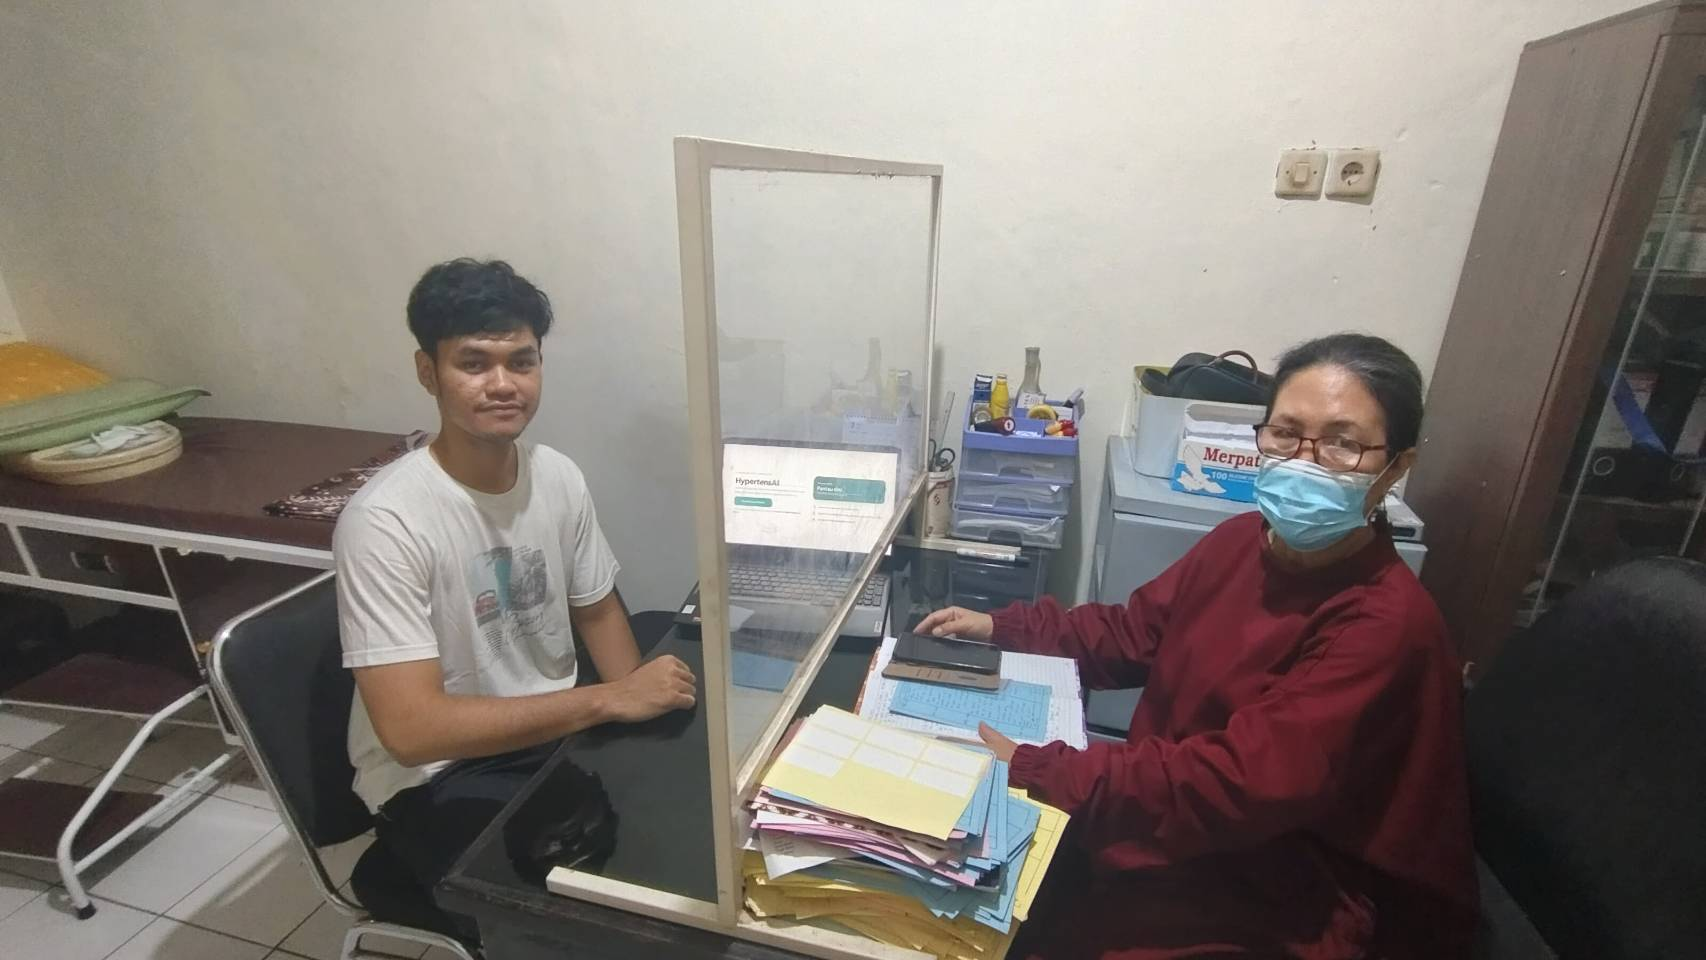
\includegraphics[width=0.8\textwidth]{images/gambar2eval.jpg} 
    \caption{Dokumentasi Evaluasi 1}
    \label{fig:evaluasi1}
\end{figure}

\vspace{1cm}

\begin{figure}[htbp]
    \centering
    % Masukkan path/nama file gambar kedua di bawah ini
    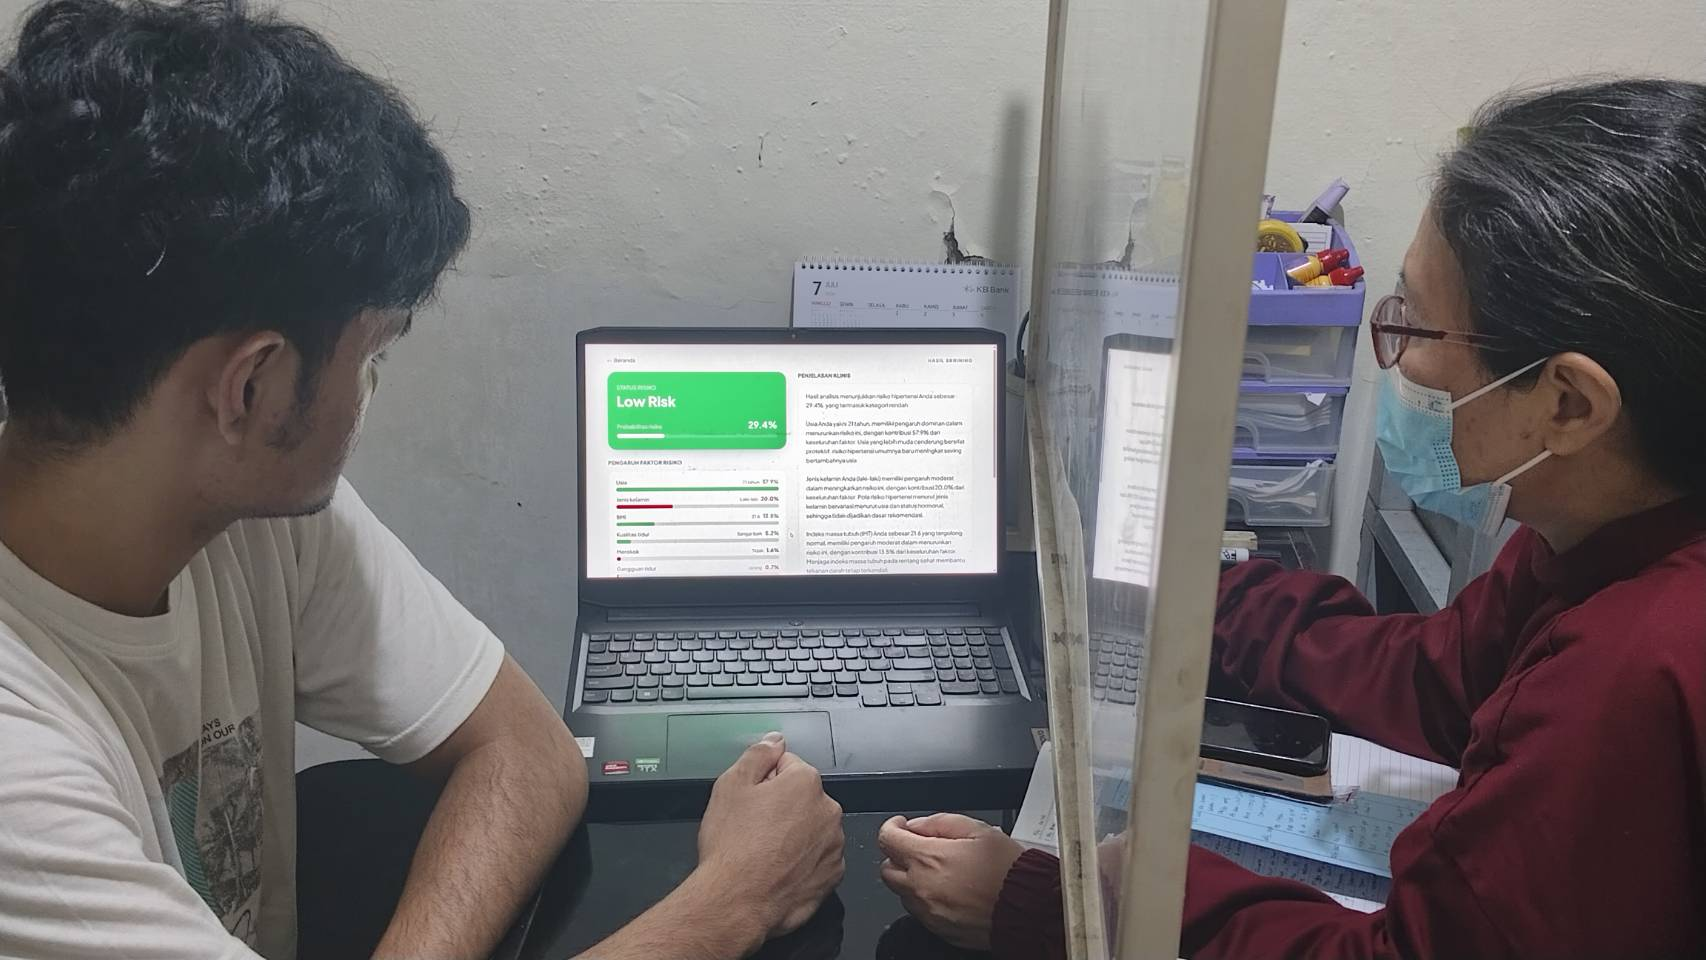
\includegraphics[width=0.8\textwidth]{images/gambar1eval.jpg}
    \caption{Dokumentasi Evaluasi 2}
    \label{fig:evaluasi2}
\end{figure}